\subsection{Quy trình đăng ký Host và công bố không gian}
\subsubsection{Nộp hồ sơ và xét duyệt quyền Host}
Tài khoản GUEST đang hoạt động mở đơn xin quyền Host, khai báo thông tin liên hệ, loại tổ chức và hai ảnh giấy tờ DEMO. Ứng dụng kiểm tra tệp, tải ảnh và gửi URL cùng hồ sơ; kết quả nộp thành công là đơn PENDING, chưa có quyền đăng phòng. Dữ liệu giấy tờ dùng trong đồ án không chứng minh danh tính pháp lý ngoài thực tế.

Admin mở hàng đợi hồ sơ trong Hình~\ref{fig:admin-application-evidence}(a), xem nội dung và ảnh trước khi quyết định. Chấp thuận cập nhật đồng thời đơn APPROVED, quyền HOST, bản chiếu PublicHost và audit. Từ chối lưu lý do để người nộp bổ sung và gửi lại theo điều kiện của đơn.

Hình~\ref{fig:host-role-transition} ghi nhận cùng một tài khoản DEMO trước và sau khi được cấp quyền. Ban đầu, hồ sơ hiển thị vai trò người thuê và lối vào đăng ký Host; sau xét duyệt, tài khoản mở được kênh người cho thuê. Quyền mới bổ sung khả năng quản lý không gian, đồng thời vẫn cho phép chuyển sang giao diện thuê.

\begin{figure}[H]\centering
\begin{minipage}[t]{0.34\linewidth}\centering
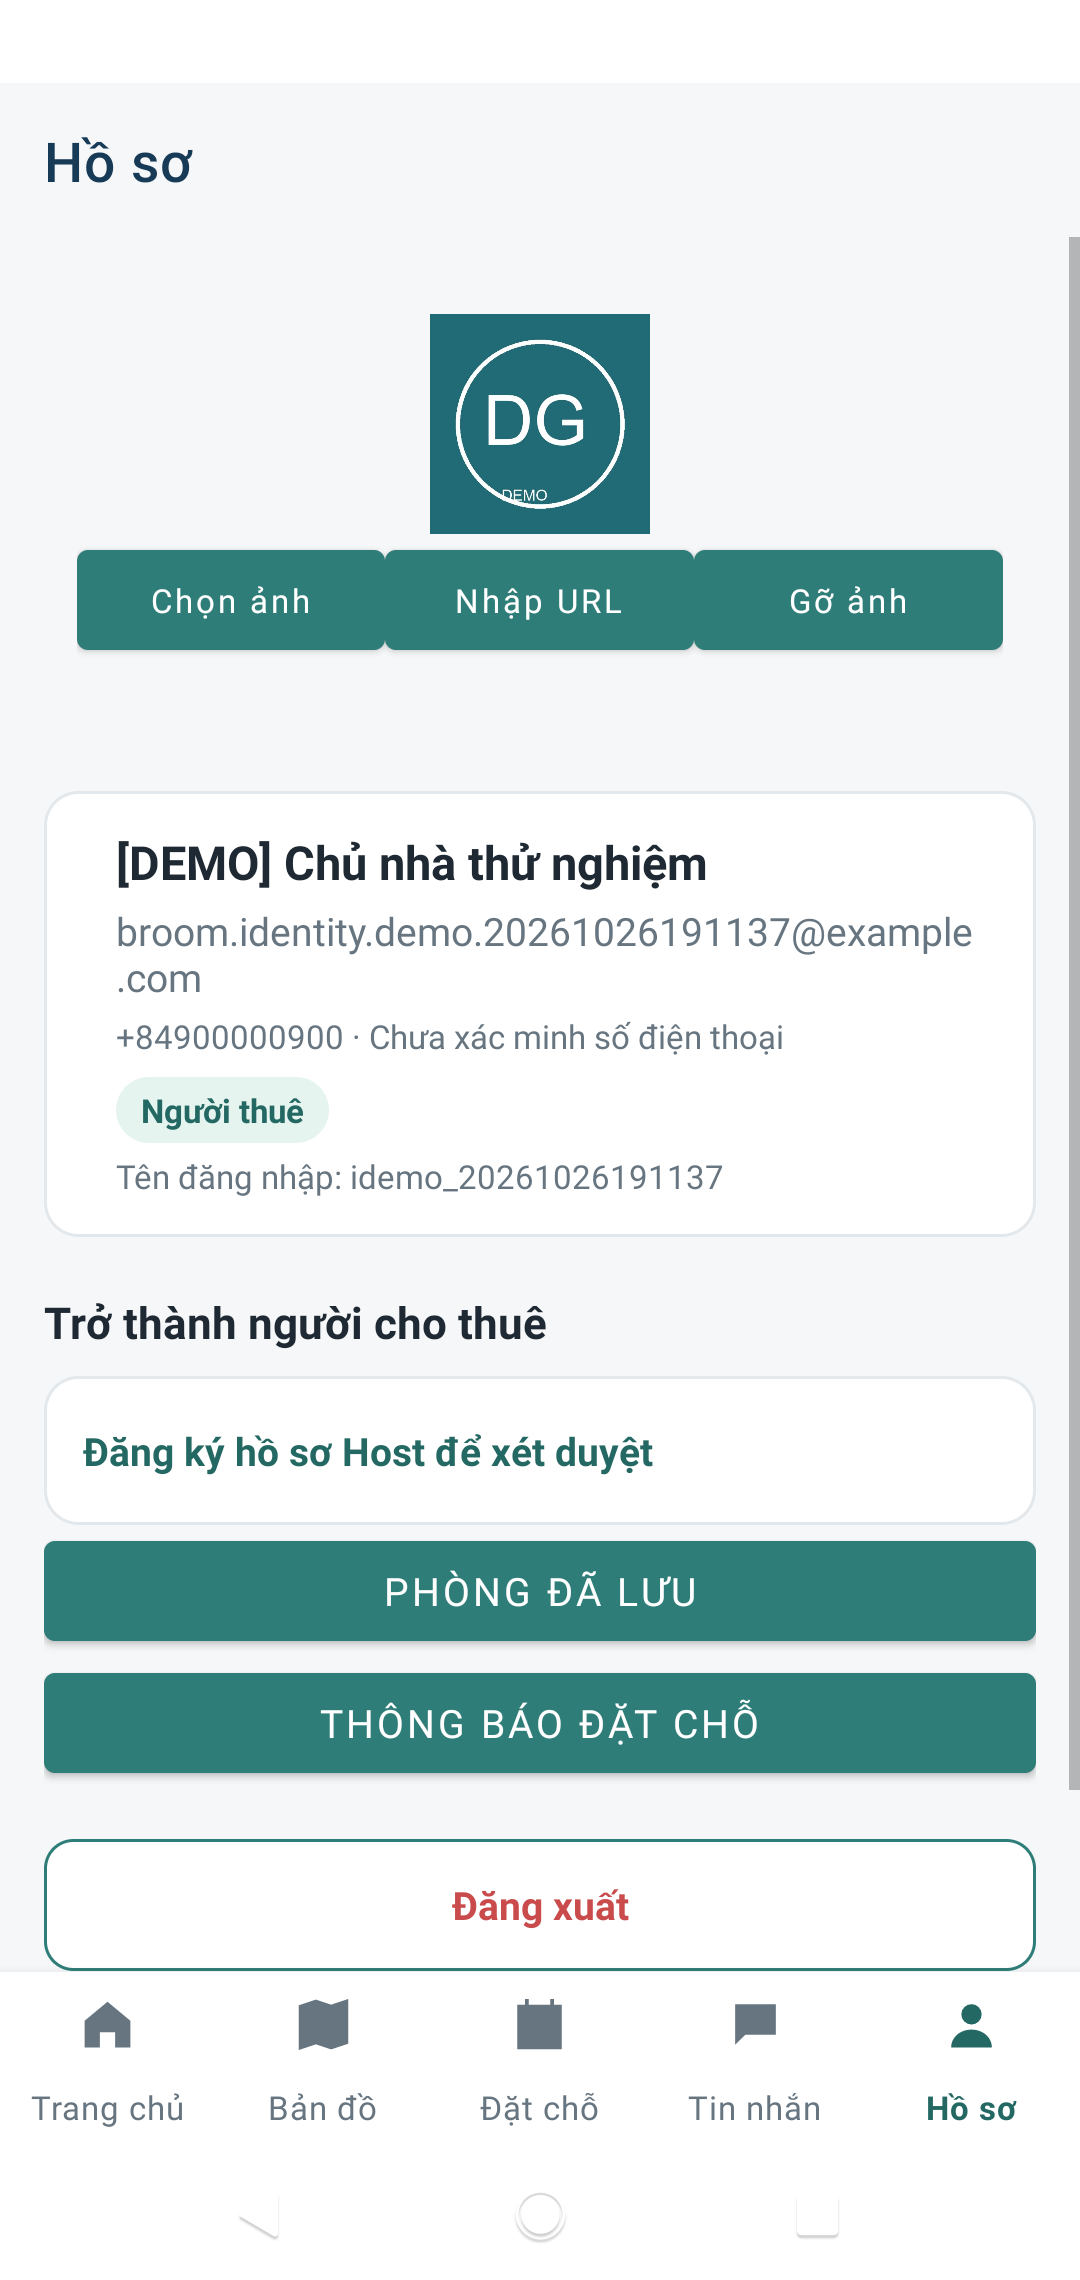
\includegraphics[width=\linewidth]{chapter6/host-role-before.png}\\[-1mm]
{\small (a) Trước khi được cấp quyền}
\end{minipage}\hspace{0.05\linewidth}%
\begin{minipage}[t]{0.34\linewidth}\centering
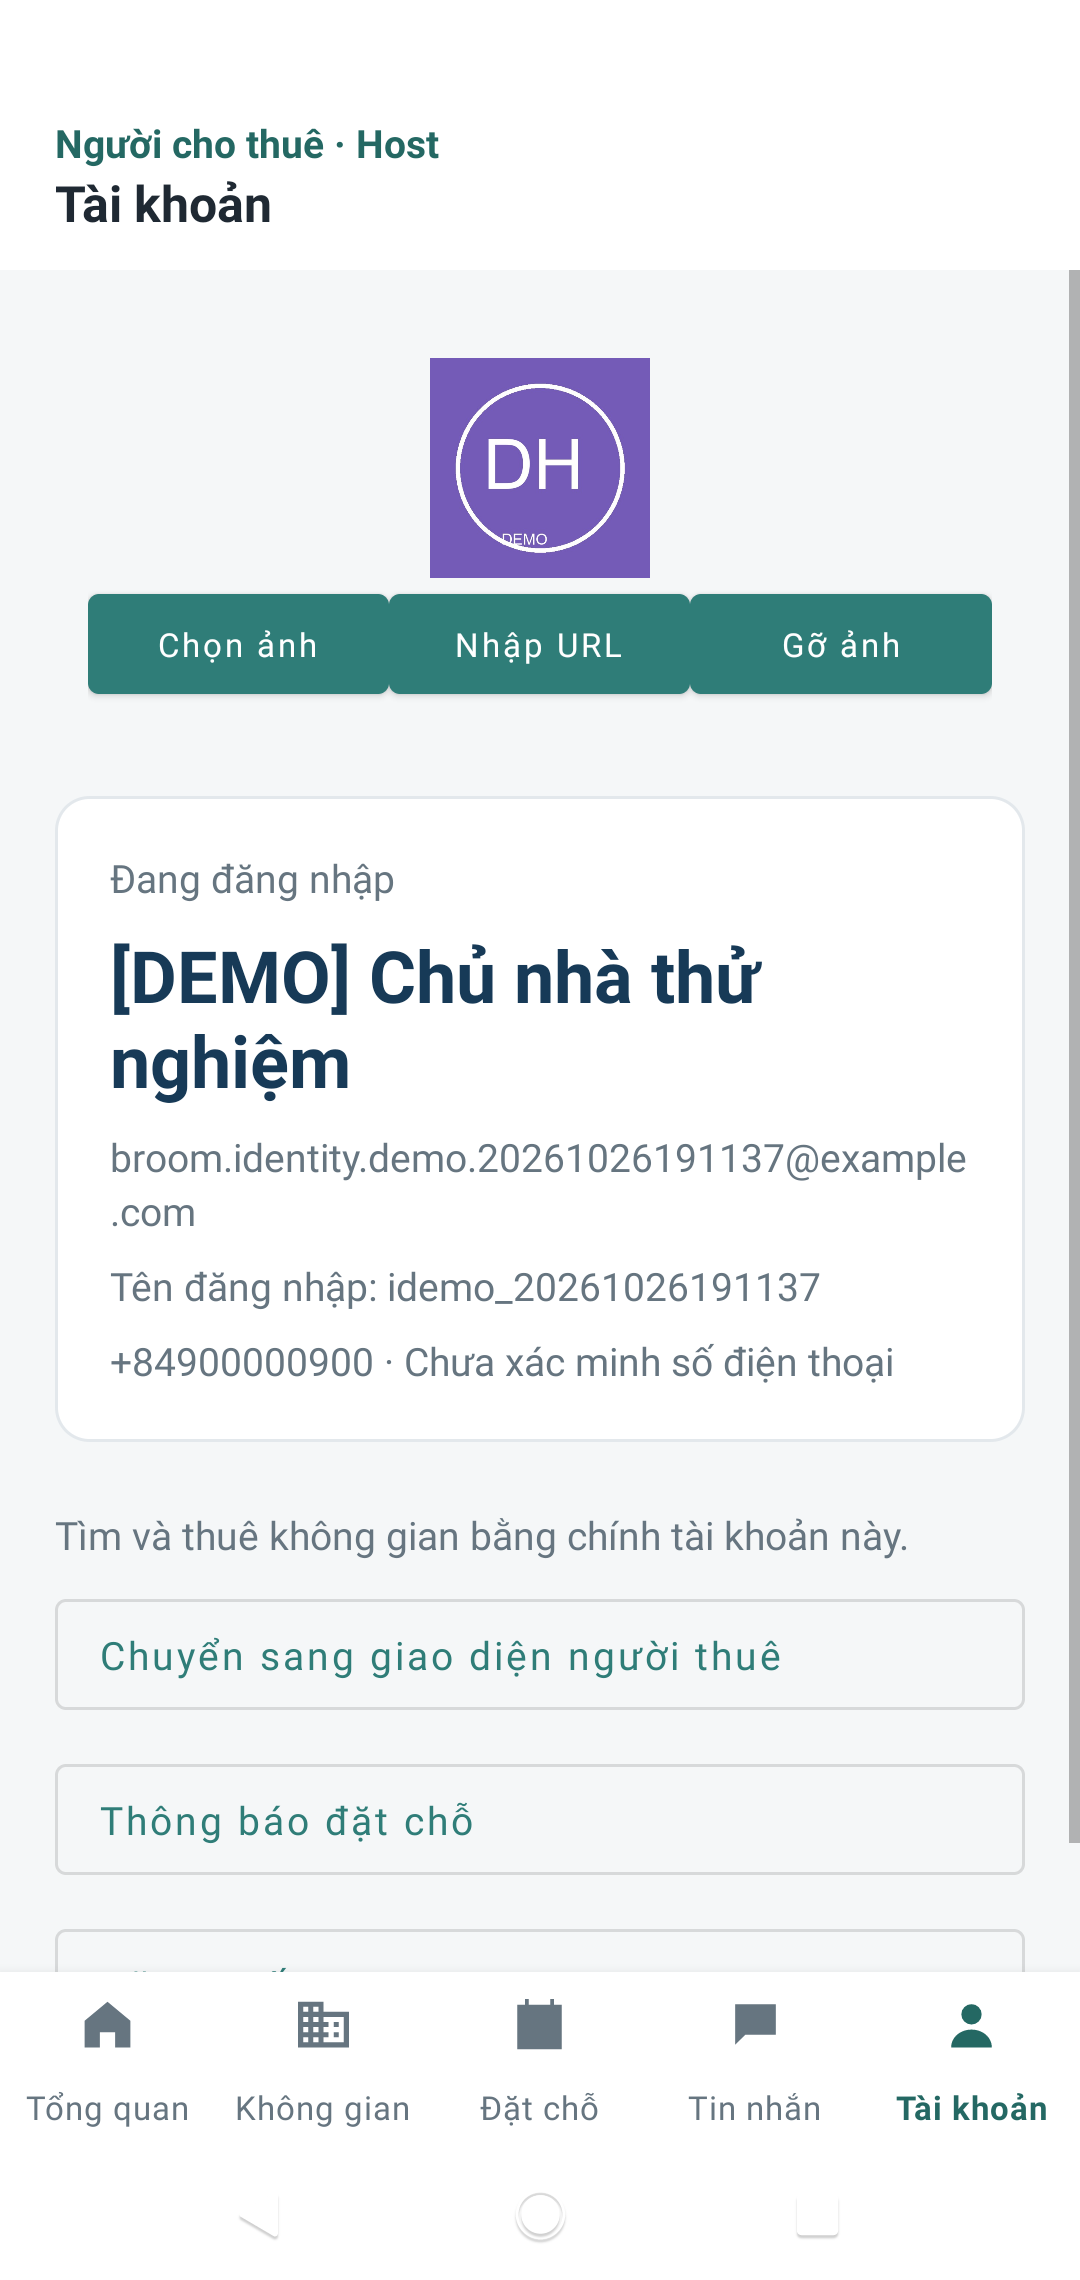
\includegraphics[width=\linewidth]{chapter6/host-role-after.png}\\[-1mm]
{\small (b) Tài khoản đã có quyền Host}
\end{minipage}
\caption{Thay đổi quyền của tài khoản sau quy trình xét duyệt Host}
\label{fig:host-role-transition}
\end{figure}

\Needspace{9\baselineskip}
\subsubsection{Tạo, xét duyệt và công bố không gian}
Sau khi được cấp quyền, Host thực hiện trình tự sau:
\begin{enumerate}
\item Tạo tòa nhà với địa chỉ, liên hệ và vị trí; sau đó mở biểu mẫu phòng, chọn tòa nhà thuộc sở hữu và nhập thông tin cơ bản, ảnh, tiện ích.
\item Chọn thuê giờ hoặc tháng/quý, thiết lập giá và lịch phù hợp. Kiểm tra ngày làm việc, khung giờ, thời lượng tối thiểu hoặc tháng bắt đầu thuê cố định; lưu nháp nếu chưa hoàn tất.
\item Gửi bài đăng xét duyệt. Admin đọc thông tin phòng và đối tượng liên quan, chấp thuận hoặc từ chối kèm lý do. Host theo dõi kết quả và mở cho thuê khi đáp ứng điều kiện.
\end{enumerate}

Phòng chỉ xuất hiện với người thuê khi APPROVED và ACTIVE. Duyệt đơn Host không tự duyệt phòng; xét duyệt minh chứng vị trí/ảnh cũng là hồ sơ riêng. Khi sửa cấu hình có ảnh hưởng lịch, hệ thống kiểm tra các booking đang giữ chỗ để bảo toàn kỳ thuê đã đặt. Hình~\ref{fig:actual-host-editor} minh họa dữ liệu đầu vào, còn Hình~\ref{fig:admin-overview-review} thể hiện bước xét duyệt tin đăng.

Hình~\ref{fig:room-publication-stages} minh họa cách Host theo dõi kết quả công bố theo từng phòng. Nhãn đã duyệt và đang hiển thị được đặt trên thẻ phòng; các nút chỉnh sửa và lịch đặt mở thao tác tương ứng. Màn Admin tại Hình~\ref{fig:admin-overview-review}(b) thực hiện bước xét duyệt riêng; việc duyệt tin đăng độc lập với xác nhận booking sau thanh toán.

\begin{figure}[H]\centering
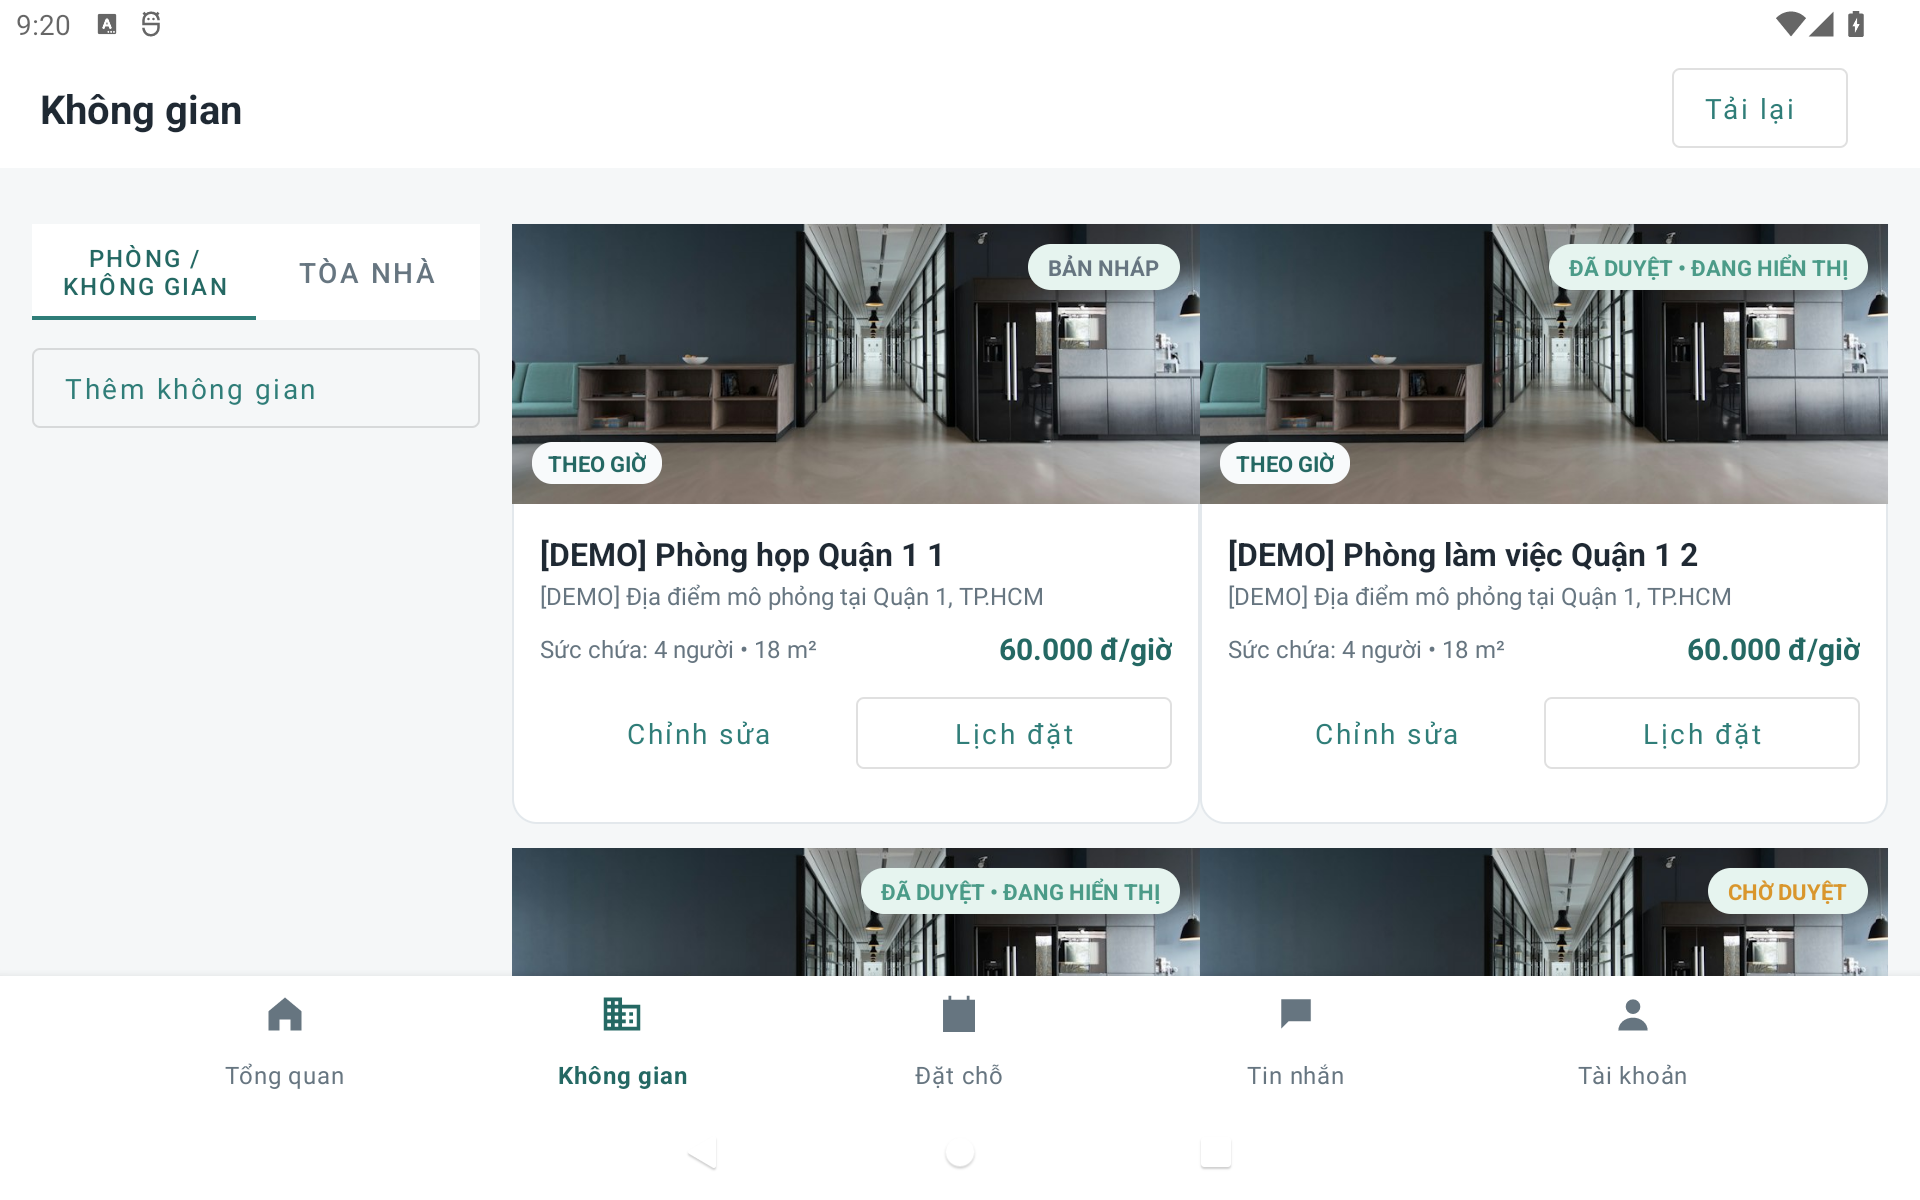
\includegraphics[width=0.96\linewidth]{chapter5/members/host-tablet-spaces-landscape.png}
\caption{Host theo dõi trạng thái công bố và thao tác trên từng phòng}
\label{fig:room-publication-stages}
\end{figure}
